\documentclass[14pt]{article}
\usepackage[utf8]{inputenc}
\usepackage[T2A]{fontenc}
\usepackage[russian]{babel}
\usepackage{amsmath, amssymb}
\usepackage{geometry}
\usepackage{graphicx}
\usepackage{xcolor}
\usepackage{hyperref}
\usepackage{tasks}
\usepackage{tcolorbox}
\tcbuselibrary{skins, breakable}
\usepackage{fancyhdr}
\usepackage{lastpage}
\usepackage{enumitem}

% Определение команд для тангенса и котангенса (русский стиль)
\newcommand{\tg}{\operatorname{tg}}
\newcommand{\ctg}{\operatorname{ctg}}

% Настройка геометрии
\geometry{a4paper, left=20mm, right=15mm, top=25mm, bottom=25mm, headheight=20pt}

% Цвета
\definecolor{taskblue}{RGB}{0, 102, 204}
\definecolor{lightorange}{RGB}{255, 240, 220}
\pagecolor{lightorange!10}

\newtcolorbox[auto counter]{taskbox}[1][]{
  colback=white,
  colframe=taskblue,
  arc=5pt,
  boxrule=1.5pt,
  left=8pt,
  right=8pt,
  top=8pt,
  bottom=8pt,
  fonttitle=\bfseries\large,
  title=Задача \thetcbcounter,
  breakable,
  pad at break=2mm,
  #1
}
% Настройка tasks (варианты ответов в две колонки)
\settasks{
  label=\Alph*),
  label-width=1.8em,
  item-indent=2.5em,
  column-sep=2em,
  before-skip=3pt,
  after-skip=3pt
}

% Колонтитулы
\pagestyle{fancy}
\fancyhf{}
\fancyhead[L]{\textbf{MathCore} | MOCK Test-4}
\fancyhead[R]{Abdunazarov M.X.}
\fancyfoot[L]{\href{https://t.me/Math_Core_Dtm_MS_Att}{\textbf{MathCore}}}
\fancyfoot[R]{\href{https://t.me/Abd_mardon}{\textbf{@Abd\_mardon}}}
\fancyfoot[C]{\thepage/\pageref{LastPage}}
\renewcommand{\headrulewidth}{0.4pt}
\renewcommand{\footrulewidth}{0.4pt}

% Титульная страница
\title{\Huge \textbf{MOCK Test-4}}
\author{Abdunazarov M.X.}
\date{}

\begin{document}

\maketitle

\begin{center}
    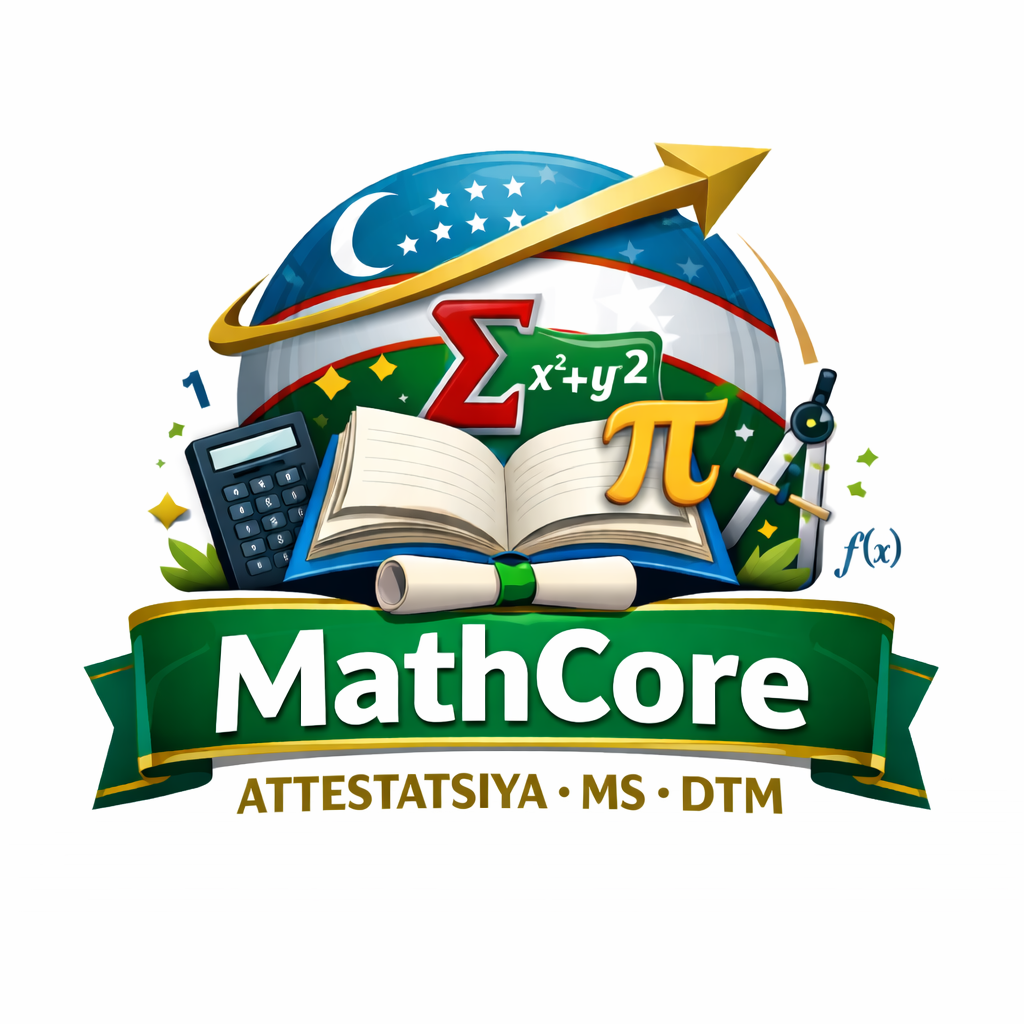
\includegraphics[width=0.3\textwidth]{logo.png} 
\end{center}
\vspace{1cm}

% Задача 1
\begin{taskbox}
Наргиза решила 46 задач. За каждый правильный ответ ей начисляют 5 баллов, а за каждый неправильный ответ вычитают 12 баллов. Если она набрала 77 баллов, сколько задач она решила правильно?
\begin{tasks}(2)
\task 43
\task 41
\task 39
\task 37
\end{tasks}
\end{taskbox}

% Задача 2
\begin{taskbox}
Двое рабочих вместе выполняют работу за 12 дней. Если первый рабочий выполнит половину работы, а затем второй выполнит оставшуюся половину, то они закончат за 25 дней. Во сколько раз первый рабочий работает быстрее второго?
\begin{tasks}(2)
\task 2
\task 1,5
\task 1,8
\task 2,5
\end{tasks}
\end{taskbox}

% Задача 3
\begin{taskbox}
Объем прямой призмы равен 40. В нее вписан шар объемом $\frac{32\pi}{3}$. Найдите площадь боковой поверхности призмы.
\begin{tasks}(2)
\task 10
\task 30
\task 40
\task 60
\end{tasks}
\end{taskbox}

% Задача 4
\begin{taskbox}
Первый и второй рабочие выполняют работу за 8 часов, первый и третий – за 12 часов, второй и третий – за 24 часа. За сколько часов выполнят работу все трое вместе?
\begin{tasks}(2)
\task 6
\task 16
\task 12
\task 8
\end{tasks}
\end{taskbox}

% Задача 5
\begin{taskbox}
Сколько решений имеет уравнение $\tg 2x = \ctg 4x$ на отрезке $[0; \pi]$?
\begin{tasks}(2)
\task 3
\task 4
\task 5
\task 6
\end{tasks}
\end{taskbox}

% Задача 6
\begin{taskbox}
Решите неравенство: $|\lg x| < 1$.
\begin{tasks}(2)
\task $(10^{-1}; 10)$
\task $(0; 10)$
\task $(1; 10)$
\task $(10^{-2}; 10^{-1})$
\end{tasks}
\end{taskbox}

% Задача 7
\begin{taskbox}
Уравнение $\lg x + \lg(x+6) = \lg(-a)$. При каких значениях $a$ уравнение имеет единственное решение?
\begin{tasks}(2)
\task $\varnothing$
\task $a < 0$
\task $a \in \mathbb{R}$
\task $a \in (-7; 0)$
\end{tasks}
\end{taskbox}

% Задача 8
\begin{taskbox}
Сколько целых решений имеет уравнение $\sin 4\pi x + \sin 2\pi x = 0$ на отрезке $[0, 2\pi]$?
\begin{tasks}(2)
\task 1
\task 3
\task 5
\task 7
\end{tasks}
\end{taskbox}

% Задача 9
\begin{taskbox}
Найдите остаток от деления $7^{201}$ на 23.
\begin{tasks}(2)
\task 1
\task 11
\task 17
\task 21
\end{tasks}
\end{taskbox}


\begin{taskbox}
Найдите угол $\alpha$.
\begin{center}
    \centering
    
\includegraphics[width=0.5\linewidth]{3.png}
\end{center}
\begin{tasks}(2)
\task $40^\circ$
\task $25^\circ$
\task $50^\circ$
\task $10^\circ$
\end{tasks}
\end{taskbox}


% Задача 10
\begin{taskbox}
Разложите на множители: $(a+b+c)(ab+bc+ac) - abc$.
\begin{tasks}(2)
\task $(a+b)(b+c)(a+c)$
\task $(a+b+c)^2$
\task $(a+b+c)(a+b-c)$
\task $(a+b)(ab+bc+ac)$
\end{tasks}
\end{taskbox}

% Задача 11
\begin{taskbox}
Уравнение $|7 - 6x - x^2| = 5a$. При каких значениях $a$ уравнение имеет 3 решения?
\begin{tasks}(2)
\task $a \in (0; 3,2)$
\task $a = 3,2$
\task $a > 3,2$
\task $a = 0$
\end{tasks}
\end{taskbox}

% Задача 12
\begin{taskbox}
Если $a, b, c$ — различные цифры, и для них выполняется равенство $\overline{aabc} = (a+b+c)^3$, где $\overline{aabc}$ — четырехзначное число, то найдите значение $a+b-c$.
\begin{tasks}(2)
\task 8
\task 6
\task 4
\task 5
\end{tasks}
\end{taskbox}

% Задача 13
\begin{taskbox}
В равнобедренном треугольнике высота, опущенная на основание, равна 20, а основание равно 30. Найдите высоту, опущенную на боковую сторону.
\begin{tasks}(2)
\task 25
\task 24
\task 15
\task 18
\end{tasks}
\end{taskbox}



% Задача 15
\begin{taskbox}
Из системы уравнений найдите значение $xyz$:
\[
\begin{cases}
x + y + z = 6\\
x - y + z = 4\\
z + y - x = 0
\end{cases}
\]
\begin{tasks}(2)
\task 2
\task 4
\task 6
\task 0
\end{tasks}
\end{taskbox}

% Задача 16
\begin{taskbox}
46 учеников отправились на 10 лодках. Если лодки были 6-местные и 4-местные, сколько учеников плыло на 4-местных лодках?
\begin{tasks}(2)
\task 7
\task 6
\task 24
\task 28
\end{tasks}
\end{taskbox}

% Задача 17
\begin{taskbox}
Сколько двузначных чисел не делятся ни на 3, ни на 4?
\begin{tasks}(2)
\task 50
\task 46
\task 40
\task 52
\end{tasks}
\end{taskbox}

% Задача 18
\begin{taskbox}
Ряд натуральных чисел разбит на группы, каждая из которых заканчивается квадратом натурального числа: $\{1\}$, $\{2;3;4\}$, $\{5;6;7;8;9\}$, $\{10;11;12;13;14;15;16\}$, ... Найдите сумму чисел в 10-й группе.
\begin{tasks}(2)
\task 1626
\task 1729
\task 1758
\task 1800
\end{tasks}
\end{taskbox}


\begin{taskbox}
Найдите расстояние от центра окружности до точки B.
\begin{center}
    \centering
    
\includegraphics[width=0.4\linewidth]{2.png}
\end{center}
\begin{tasks}(2)
\task 15
\task 14
\task 13
\task 12
\end{tasks}
\end{taskbox}

% Задача 19
\begin{taskbox}
Найдите область значений функции $y = \lg(\cos x)$.
\begin{tasks}(2)
\task $E(y) = (-\infty; 0]$
\task $E(y) = (-1; 0]$
\task $E(y) = (0; \infty)$
\task $E(y) = (-\infty; \infty)$
\end{tasks}
\end{taskbox}

% Задача 20
\begin{taskbox}
Сколько острых углов (т.е. $x \in (0; \frac{\pi}{2})$) удовлетворяет уравнению $\sin 4x + \cos 2x = 0$?
\begin{tasks}(2)
\task 1
\task 2
\task 3
\task 4
\end{tasks}
\end{taskbox}

% Задача 21
\begin{taskbox}
Вычислите: $\dfrac{3\lg 2 + 3\lg 5}{\lg 1300 - \lg 0,13}$.
\begin{tasks}(2)
\task $1,5$
\task $1,25$
\task $0,75$
\task $0,5$
\end{tasks}
\end{taskbox}

% Задача 22
\begin{taskbox}
Найдите сумму корней уравнения $\tg 2x = \ctg 4x$ на отрезке $[0; \pi]$.
\begin{tasks}(2)
\task $\dfrac{35\pi}{12}$
\task $\dfrac{11\pi}{4}$
\task $2\pi$
\task $\dfrac{13\pi}{6}$
\end{tasks}
\end{taskbox}

% Задача 23
\begin{taskbox}
Найдите область значений функции $y = \lg(\arcsin x)$.
\begin{tasks}(2)
\task $E(y) = (-\infty; \lg 2]$
\task $E(y) = (-\infty; 0]$
\task $E(y) = (0; \infty)$
\task $E(y) = (-\infty; \infty)$
\end{tasks}
\end{taskbox}

% Задача 24
\begin{taskbox}
Радиусы оснований усеченного конуса равны 11 и 27. Отношение образующей к высоте равно $17:15$. Найдите площадь осевого сечения.
\begin{tasks}(2)
\task 760
\task 1140
\task 1260
\task 1440
\end{tasks}
\end{taskbox}

% Задача 14
\begin{taskbox}
В равнобедренном треугольнике боковая сторона равна 15, а высота, опущенная на основание, равна 12. Найдите длину высоты, опущенной на боковую сторону.
\begin{tasks}(2)
\task 14,4
\task 15
\task 16,2
\task 18
\end{tasks}
\end{taskbox}

% Задача 25
\begin{taskbox}
Найдите область значений функции $y = |x-1| + |x-3|$.
\begin{tasks}(2)
\task $E(y) = (2; \infty]$
\task $E(y) = (-\infty; 0]$
\task $E(y) = [2; \infty)$
\task $E(y) = (-\infty; \infty)$
\end{tasks}
\end{taskbox}

% Задача 26
\begin{taskbox}
Объем прямой призмы равен 40, а объем вписанного в нее шара равен $\frac{32\pi}{3}$. Найдите отношение площади боковой поверхности призмы к площади поверхности шара.
\begin{tasks}(2)
\task $\dfrac{10}{5\pi}$
\task $\dfrac{10}{3\pi}$
\task $\dfrac{5}{2\pi}$
\task $\dfrac{5}{2\pi}$
\end{tasks}
\end{taskbox}

% Задача 27
\begin{taskbox}
Сколько целых решений имеет неравенство $1 < |x-2| < 3$?
\begin{tasks}(2)
\task 0
\task 1
\task 2
\task 3
\end{tasks}
\end{taskbox}

% Задача 26
\begin{taskbox}
Точка G является центром тяжести треугольника ABC. Найдите площадь треугольника BGC если $AG \perp CG, \ CG=15, \ BG=20$.
\begin{center}
    \centering
    
\includegraphics[width=0.5\linewidth]{1.png}
\end{center}
\begin{tasks}(2)
\task $\dfrac{75\sqrt{7}}{2}$
\task $\dfrac{77\sqrt{7}}{2}$
\task $36\sqrt{5}$
\task $37\sqrt{5}$
\end{tasks}
\end{taskbox}

% Задача 28
\begin{taskbox}
Сколько решений имеет уравнение $|x|(x^2 - 4) = -1$?
\begin{tasks}(2)
\task 1
\task 2
\task 3
\task 4
\end{tasks}
\end{taskbox}
\begin{taskbox}
В треугольнике $ABC$, $BD$ --- биссектриса, $\angle BAC = 30^{\circ}$, $\angle BCA = 45^{\circ}$ и $DC = 8\sqrt{2}$. Найдите длину отрезка $AD$.
\begin{center}
    \centering
    
\includegraphics[width=0.5\linewidth]{4.png}
\end{center}
\begin{tasks}(2)
\task 12
\task 14
\task 16
\task \(16 \sqrt{2}\)
\end{tasks}

\end{taskbox}

% Задача 29
\begin{taskbox}
Даны два конуса с основаниями, лежащими в параллельных плоскостях, и общей высотой. Радиусы оснований равны 4 и 6. Если $H = 15$, найдите объем общей части конусов.
\begin{tasks}(2)
\task $\dfrac{144\pi}{5}$
\task $40\pi$
\task $\dfrac{216\pi}{5}$
\task $60\pi$
\end{tasks}
\end{taskbox}

% Задача 30
\begin{taskbox}
Найдите площадь треугольника, медианы которого равны 9, 12 и 15.
\begin{tasks}(2)
\task 80
\task 72
\task 64
\task 60
\end{tasks}
\end{taskbox}



% Задача 2
\begin{taskbox}
Дан правильный треугольник $ABC$. На стороне $AC$ отмечены точки $K$ и $L$ так, что $AK = KL = LC = 4$. Найдите площадь закрашенной области.
\begin{center}
    \centering
    
\includegraphics[width=0.4\linewidth]{5.png}
\end{center}
\begin{tasks}(2)
\task \(12 \sqrt{3}\)
\task \(15 \sqrt{3}\)
\task \(18 \sqrt{3}\)
\task \(24 \sqrt{3}\)
\end{tasks}
\end{taskbox}
\end{document}